%chapter{Design Methodology}
%\label{chap:4}

%NS3
%System Design
%Methodology
%Architecture

%\todo[inline]{I suggest that you add a figure that explains how all these definitions (symbols and blocks) are connected to each others. Also, you should detail more (use examples if necessary)}
\hspace{\parindent} The performance evaluation of ALFEC--UDP was carried out through simulation using network simulation (ns-3). In this chapter, ns-3 is described briefly in section \ref{ns3}. In sections \ref{sys_design_sec} and \ref{methodology_} system design and the methodology that has been employed for building ALFEC--UDP is explained.

\section{Network Simulator-3}
\label{ns3}
Network Simulator-3 is a discrete event network simulator used in research and education. The simulator is written from scratch using C++ and Python programming language by a team lead by Tom Henderson and funded from the U.S. National Science Foundation (NSF).

\begin{figure}[htbp]
\begin{center}
\mbox{
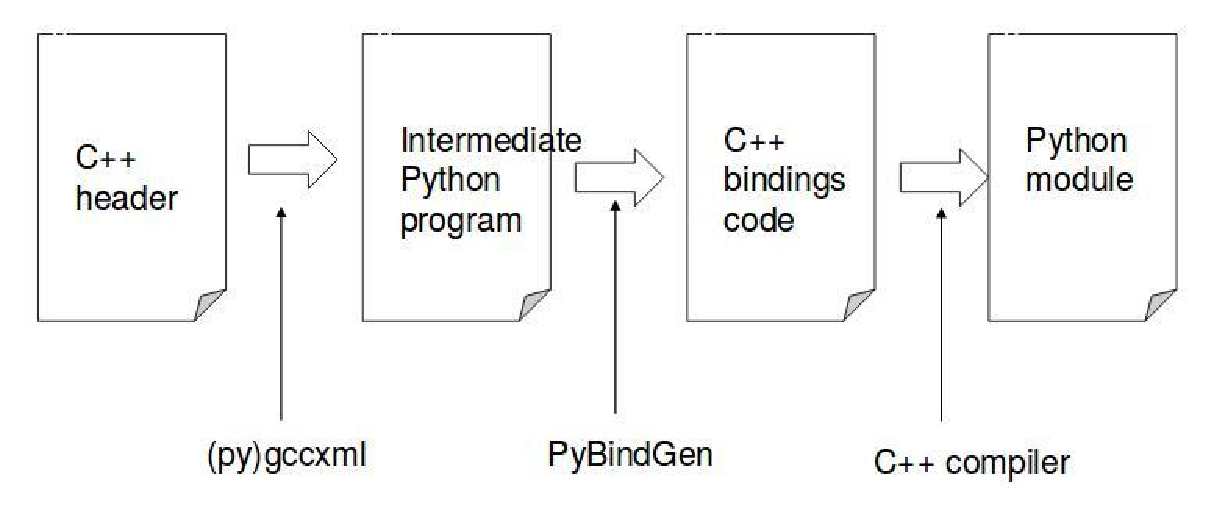
\includegraphics[width=4.5in]{Figures/python}}
\caption{PyBindGen used to generate python bindings for all libraries}
\label{python}
\end{center}
\end{figure}

The ns-3 library is wrapped by Python and the library PyBindGen is used for parsing the headers to automatically generate the corresponding C++ files. Fig \ref{python} shows how library PyBindGen helps to generate Python bindings for all libraries.

Ns-3 provides models of how packet data networks work and perform, and provides a simulation engine for users to conduct simulation experiments. Most of the ns-3 API is available in Python, but the models are written in C++. User programs can be written in both C++ and Python.

Ns-3 is organized into two-level of software and libraries. 
The one is ns-3 modules that exist within the ns-3 directory as shown in fig \ref{ns3org}. This simulator supports a series of modules such as routing protocols, ad-hoc networking, and access technologies while providing simulation results for wired and wireless networks alike. 
The other level that ns-3 supports is libraries and software that are not bound within ns-3; affording a high level of independence to researchers, allowing them the opportunity to extend the simulator by modifying the source code and to contribute to the existing module as a result of adding new functionality, thus advantageous for abstraction, emulation, scenario generation, visualization and extensibility.
\begin{figure}[htbp]
\begin{center}
\mbox{
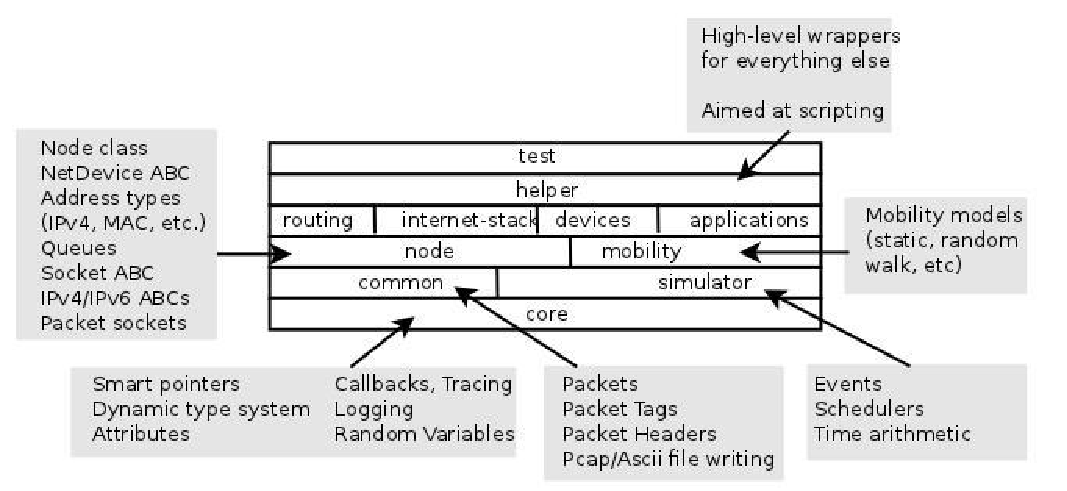
\includegraphics[width=5.5in]{Figures/ns3org}}
\caption{Organization of ns-3 modules directory}
\label{ns3org}
\end{center}
\end{figure}

\section{System Design}
\label{sys_design_sec}

In this design, UDP was selected as the transmission protocol for the purpose of data transmission at the transport layer. UDP is the best fit for this design as it avoids retransmissions and delays. As UDP does not provide reliability on the datagram delivery, measures should be taken to incorporate such reliability above the transport layer. In order to achieve reliability in UDP, techniques such as Automatic repeat reQuest (ARQ) or the FEC is to be considered \cite{farrell2006essentials}. As UDP is aimed to transmit data to a large number of users, ARQ will be less efficient; therefore, fountain codes are used above the UDP to achieve reliability. 


Raptor code is implemented at the application layer (AL). The AL sends the packets through the raptor encoders, that process the data by adding redundancy before sending to the UDP transport layer. Once this has been processed, the encoded symbols are sent to lower layers for further transport to the receiver as shown in figure \ref{sys_design1}.
%figure
\begin{figure}[!htbp]
\begin{center}
\mbox{
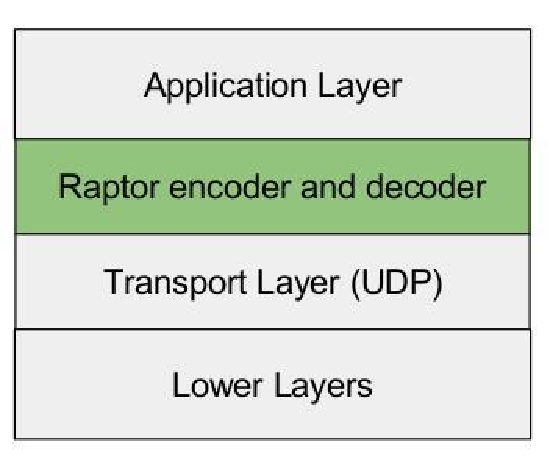
\includegraphics[width=3.0in]{Figures/sys_design}}
\caption{System Design of ALFEC--UDP}
\label{sys_design1}
\end{center}
\end{figure}
At the receiver side, the stream of encoded symbols is received from all lower layers to the AL. At this point, the encoded symbols are fed to the decoder and the data is being recovered successfully.

\section{Methodology}
\label{methodology_}
The network simulator ns-3 does not contain an implementation of the raptor FEC. Thus, the design and building a functionality module of ALFEC is necessary for ns-3. The development of the ALFEC--UDP was carried out into two stages. In the first stage, the standalone raptor FEC as described in section \ref{stand_rp} module was developed to evaluate the encoding and decoding capabilities in terms of various input parameters, overhead and file sizes. The second stage refers to the integration of raptor codes into ns-3 as explained in section \ref{ns3int}. 

As ns-3 is an integrated layering system, it allows to tightly couple the application, raptor, and transport layers. This makes raptor codes fit in between the application and the transport layer together supporting the capability of providing required information using the headers. The advantage of integrating raptor codes with ns-3 is that it would offer required visualization of network architecture and speed to run the simulation. 

\subsection{Standalone raptor FEC module}
\label{stand_rp}
The design of the standalone raptor FEC module is developed in C++ with two entities: namely encoder and decoder. The communication between the encoder and decoder did not exist directly as shown in figure \ref{stand_alone} but was established through Array\_Data\_Type class. During the standalone simulation, the binary reference of this data type of this class is passed from the encoder to the decoder.    
\begin{figure}[!htbp]
\begin{center}
\mbox{
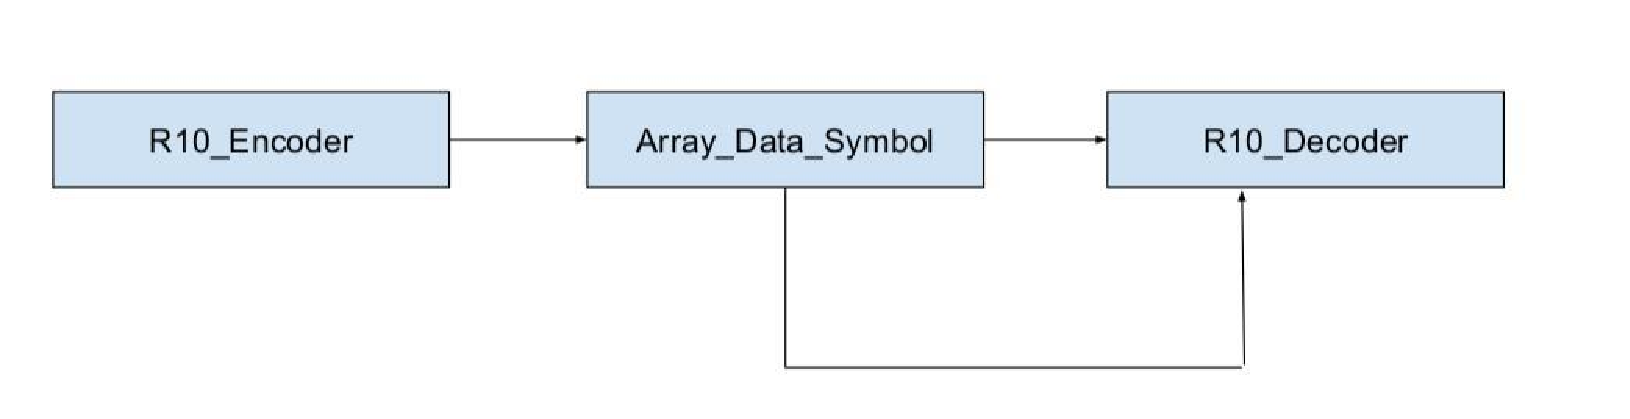
\includegraphics[width=5.2in]{Figures/stand_alone}}
\caption{Overview of raptor encoding and decoding as standalone module.}
\label{stand_alone}
\end{center}
\end{figure}
The implementation of the raptor encoder and decoder was carried out using the following classes:
\subsubsection{R10\_Encoder} \label{r10_encoder}
This class was invoked as soon as the data is made available to encode. It calls the class Array\_Data\_Type. The parameters such as \textit{K, S, H, L} representing the length of source symbols, the number of LDPC symbols, the number of Half symbols and the number of intermediate symbols for a single source block respectively are computed in Array\_Data\_Type class.

\subsubsection{Inter\_Symbol\_Generator} \label{isg}
The Inter\_Symbol\_Genrator class was used to generate the pre-code matrix, that is the intermediate symbols (or) Code Constraint Processors symbol matrix, as described in section \ref{CCP}. The matrix generated in this phase, and defined in equation \ref{eq:matrix} is stored in the data type Array\_Data\_Symbol. This matrix represents a single block of code \textit{K} and is invertible, further used for encoding the message. This matrix is a must at the receiver end to start decoding process.

\subsubsection{LT\_Encoding} \label{lte}
The LT\_Encoding class implements the LT encoding, as defined in section \ref{lt}. After the intermediate symbols are generated, the LT encoding is done by this class by XORing the intermediate symbols with degree distribution d, chosen randomly defined at section 5.4.4.2 in \cite{luby2007rfc}. Parameters, such as degree distribution, symbol length, the length of data is stored in the header of Array\_Data\_Symbol.

\subsubsection{Array\_Data\_Type} \label{adt}
The Array\_Data\_Type class serves as an intermediate link between the encoding side and the decoding side of the raptor code. The matrix, encoded symbols and other information used during encoding and decoding process are stored in Array\_Data\_type class having Array\_Data\_Symbols data type. A reference of this data type stored in a binary file and this is read by the receiver which allows the receiver to retrieve the encoded symbols generated by the encoder.

\subsubsection{R10\_Decoder} \label{r10d}
The receiver after reading the binary file converts the reference to type Array\_Data\_Symbol and then invokes the class R10\_decoder as soon as required encoded symbols are received. A subset of the matrix is used during the decoding operation to help the recovery of intermediate symbols. The retrieval of intermediate symbols operation is done by class Get\_Inter\_Symbols of type Array\_Data\_Symbols. The aim of this class is to convert the sparse matrix into identity matrix using Gaussian Elimination (GE) process. Thus, intermediate symbols would be retrieved.

The class Inter\_Symbols\_Decoding receives the intermediate symbols and performs the process of decoding to recover the original source symbols.

\subsection{Integration of raptor FEC module into ns-3}
\label{ns3int}
The first step in integration and development of ALFEC--UDP protocol was to extend the raptor standalone module as explained in section \ref{stand_rp} into the application layer of ns-3. This was done by extending the raptor module directory using the python binding script at the application level and building ns-3 again.

The second step was to define the three new packet headers at the application level. RPSendHeader, RPRecvHeader, and CDPHeader as shown in figure \ref{hdrs} were defined for the implementation of the raptor codes and were integrated into the application module of ns-3 with the application being udp-echo-client and udp-echo-server. The CDPHeader at the sender side was used to begin the communication by communicating Content Delivery Protocol (CDP) specifications fields such as total data length, number of source blocks and symbol length to the receiver. The RPSendHeader also defined at the sender side contained fields such as source block number and ESI of the packets being transferred and RPRecvHeader at the receiver was defined to acknowledge that it was ready to process the next block.
\begin{figure}[h!] 
\begin{center}
\mbox{
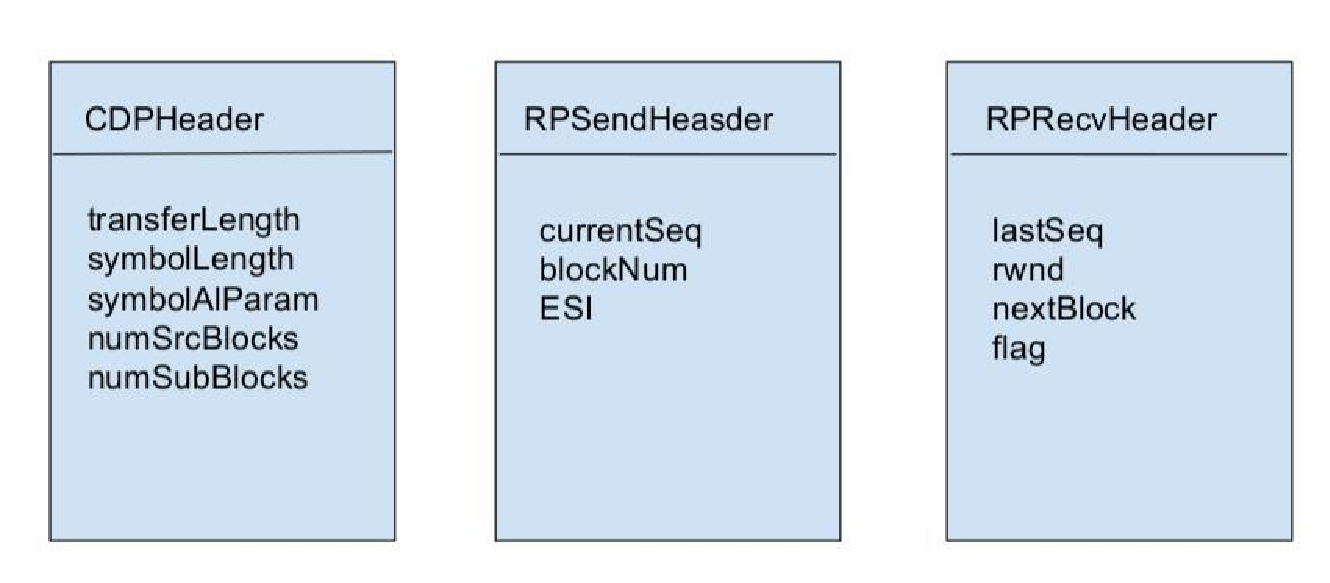
\includegraphics[width=3.7in]{Figures/hdr}}
\caption{Packet header structure}
\label{hdrs}
\end{center}
\end{figure}

After defining the headers, the following figure \ref{app} represents the structure of ALFEC--UDP protocol's packet structure used for communication in ns-3.
\begin{figure}[!htbp] 
\begin{center}
\mbox{
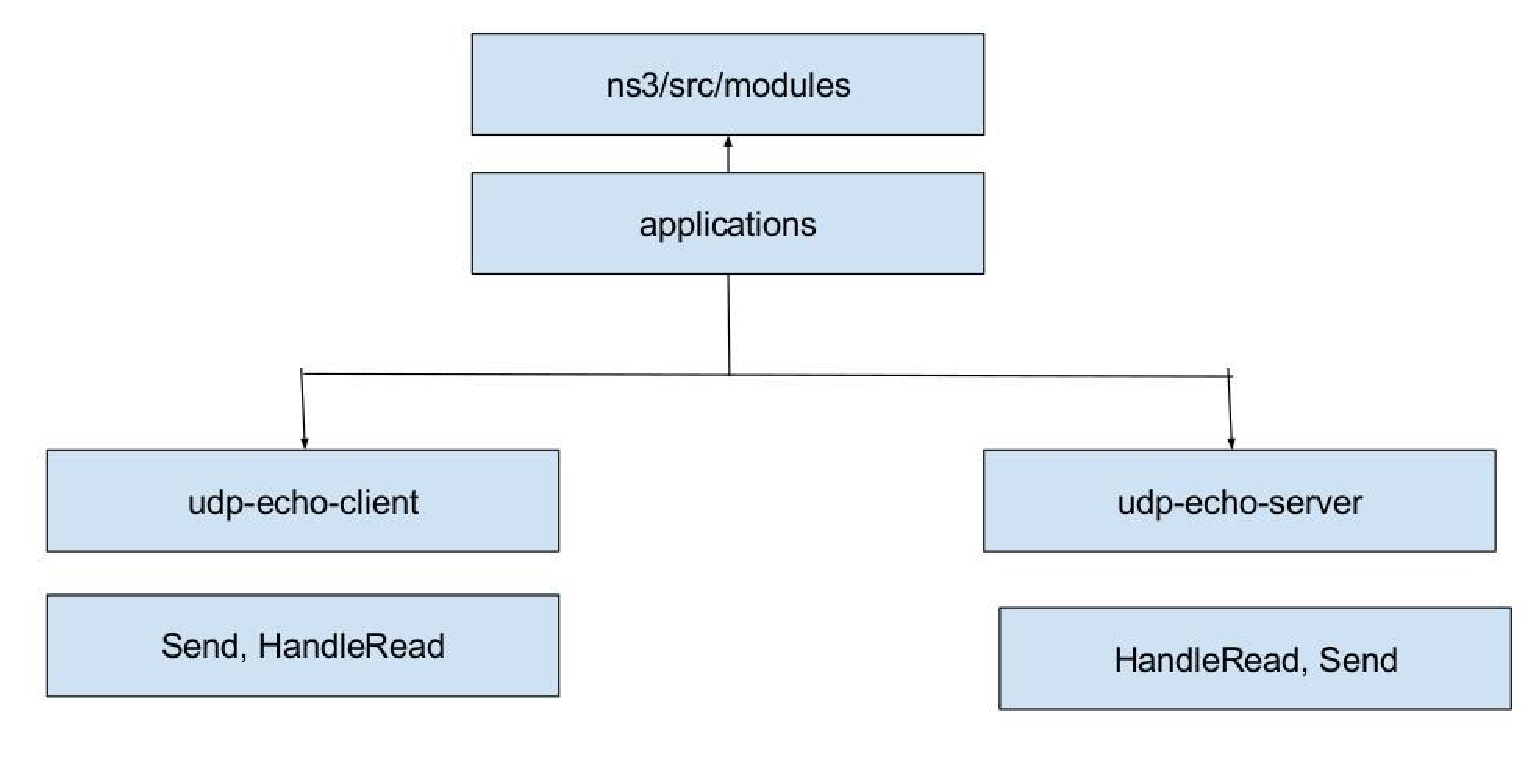
\includegraphics[width=4.0in]{Figures/app}}
\caption{Linkage of packet structure in ns-3}
\label{app}
\end{center}
\end{figure}

The functionalities of sender and receiver are separated in the course of the protocol using udp-echo-client and udp-echo-server that acts as the sender and the receiver respectively.
\subsubsection{The transmitter}
Data transmitter have three basic functionalities: namely Schedule send (Tx), wait (W), HandleRead (Rx) as shown in figure \ref{sender_flow}. 
\begin{figure}[!htbp] 
\begin{center}
\mbox{
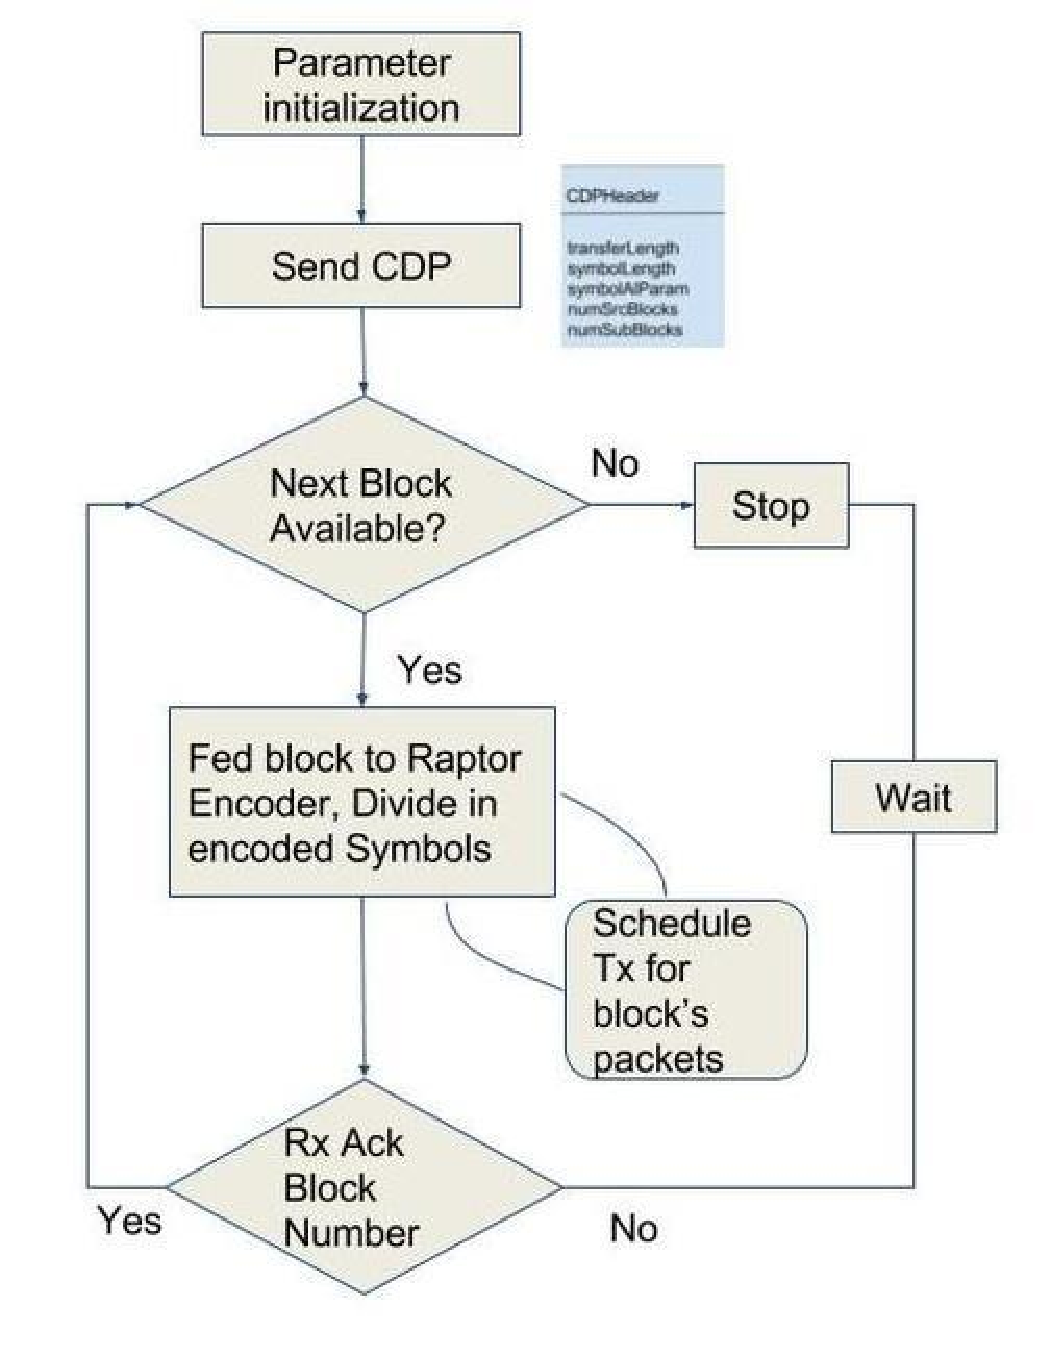
\includegraphics[width=3.5in]{Figures/rp_send}}
\caption{Transmitter side data flow}
\label{sender_flow}
\end{center}
\end{figure}
As soon as the socket is connected by the lower layers, the application layer at the sender interacts with the class Array\_Data\_Symbol to calculate the values of \textit{K, S, H, L, Z} when given the input of total data length that is to be transported. Once these parameters are calculated, the sender initiates to send CDPHeader as the first constraint to start communication. After receiving the acknowledgment by the receiver of receiving CDP specifications, the data is chunked into source blocks each of length \textit{K=1024} and fed to the R10\_Encoder and is encoded. The encoding symbols of data type Array\_Data\_Symbol are converted into packet API data type of ns-3 and are sent into the network by providing source block number and ESI for each packet using RPSendHeader. These packets are then fed to the UDP transport layer and further to the lower layers. 

\begin{figure}[!t]
\begin{center}
\mbox{
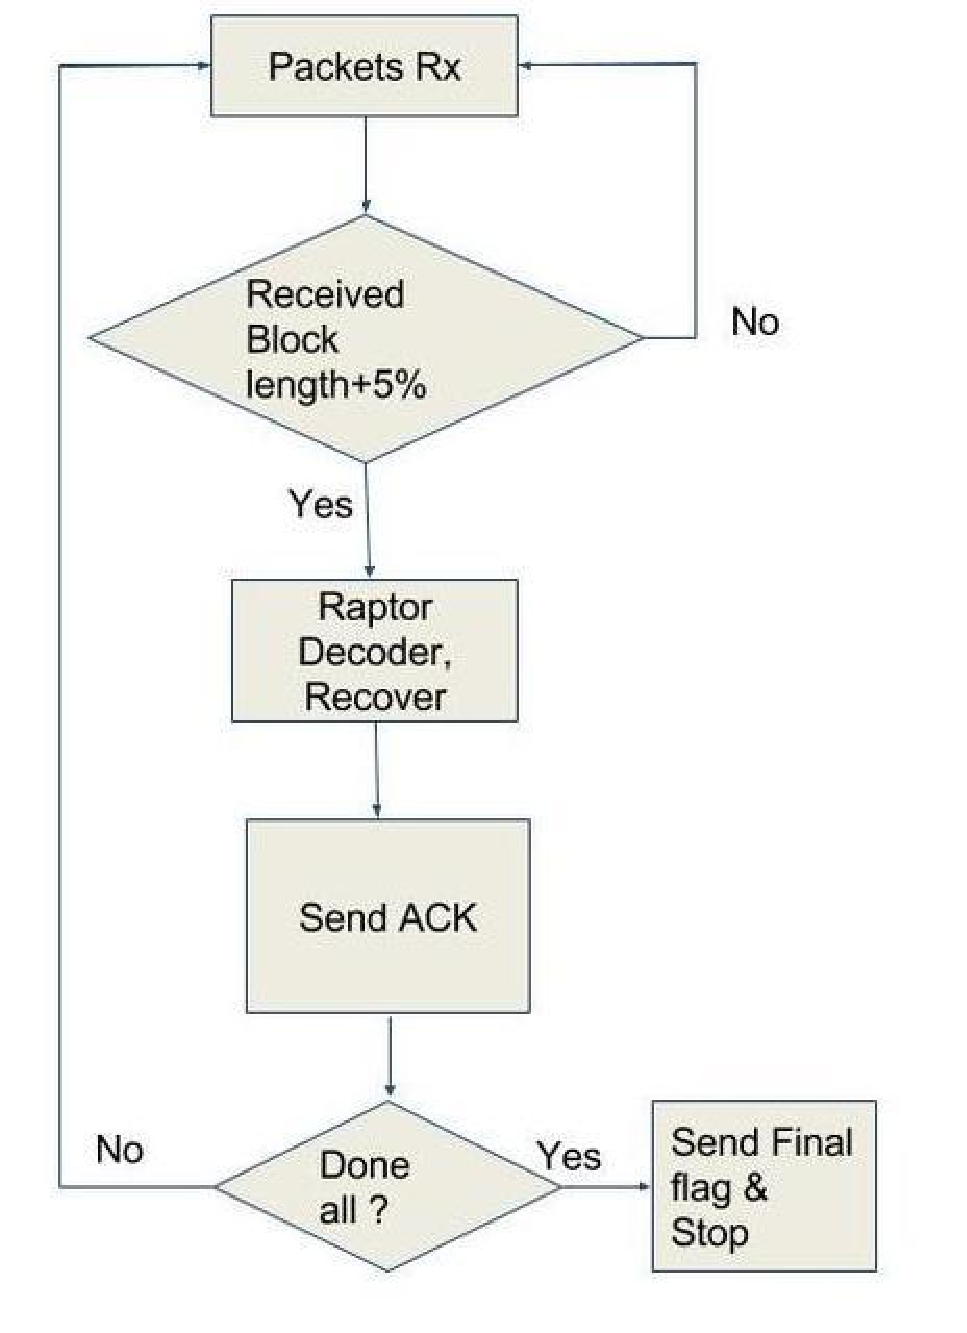
\includegraphics[width=3.0in]{Figures/rp_recv}}
\caption{Receiver side data flow}
\label{recv_flow}
\end{center}
\end{figure}

The transmitter after transmitting one chunk waits for an acknowledgment in order to process the next block. As soon as an acknowledgment is received, it then starts processing the new block. If an acknowledgment is not received it just sits in wait state until it receives an acknowledgment. 

The connection is terminated as soon as the sender receives a final acknowledgment flag from the receiver after it has successfully recovered all the original source symbols.

\subsubsection{The receiver side}
Figure \ref{recv_flow} depicts the representation of the receiver. Once the packet is received using from the sender using HandleRead (Rx) function, the encoded message is extracted from the packet. As soon as the required bytes (1.05*K) for a particular block is received, the decoding process is activated by invoking R10\_Decoder class. If the decoding process is successful, it sends an acknowledgment using the RPRecvHeader. In order for this acknowledgment to reach successfully, we make sure that it is transmitted 3 times.

As long as receiver receives the data it either will be in the receiving state or sending acknowledgment state. A final acknowledgment to terminate the connection message is sent to the sender using the \textit{flag} field in RPRecvHeader header.



               